% Options for packages loaded elsewhere
\PassOptionsToPackage{unicode}{hyperref}
\PassOptionsToPackage{hyphens}{url}
%
\documentclass[
]{article}
\usepackage{amsmath,amssymb}
\usepackage{iftex}
\ifPDFTeX
  \usepackage[T1]{fontenc}
  \usepackage[utf8]{inputenc}
  \usepackage{textcomp} % provide euro and other symbols
\else % if luatex or xetex
  \usepackage{unicode-math} % this also loads fontspec
  \defaultfontfeatures{Scale=MatchLowercase}
  \defaultfontfeatures[\rmfamily]{Ligatures=TeX,Scale=1}
\fi
\usepackage{lmodern}
\ifPDFTeX\else
  % xetex/luatex font selection
\fi
% Use upquote if available, for straight quotes in verbatim environments
\IfFileExists{upquote.sty}{\usepackage{upquote}}{}
\IfFileExists{microtype.sty}{% use microtype if available
  \usepackage[]{microtype}
  \UseMicrotypeSet[protrusion]{basicmath} % disable protrusion for tt fonts
}{}
\makeatletter
\@ifundefined{KOMAClassName}{% if non-KOMA class
  \IfFileExists{parskip.sty}{%
    \usepackage{parskip}
  }{% else
    \setlength{\parindent}{0pt}
    \setlength{\parskip}{6pt plus 2pt minus 1pt}}
}{% if KOMA class
  \KOMAoptions{parskip=half}}
\makeatother
\usepackage{xcolor}
\usepackage[margin=1in]{geometry}
\usepackage{color}
\usepackage{fancyvrb}
\newcommand{\VerbBar}{|}
\newcommand{\VERB}{\Verb[commandchars=\\\{\}]}
\DefineVerbatimEnvironment{Highlighting}{Verbatim}{commandchars=\\\{\}}
% Add ',fontsize=\small' for more characters per line
\usepackage{framed}
\definecolor{shadecolor}{RGB}{248,248,248}
\newenvironment{Shaded}{\begin{snugshade}}{\end{snugshade}}
\newcommand{\AlertTok}[1]{\textcolor[rgb]{0.94,0.16,0.16}{#1}}
\newcommand{\AnnotationTok}[1]{\textcolor[rgb]{0.56,0.35,0.01}{\textbf{\textit{#1}}}}
\newcommand{\AttributeTok}[1]{\textcolor[rgb]{0.13,0.29,0.53}{#1}}
\newcommand{\BaseNTok}[1]{\textcolor[rgb]{0.00,0.00,0.81}{#1}}
\newcommand{\BuiltInTok}[1]{#1}
\newcommand{\CharTok}[1]{\textcolor[rgb]{0.31,0.60,0.02}{#1}}
\newcommand{\CommentTok}[1]{\textcolor[rgb]{0.56,0.35,0.01}{\textit{#1}}}
\newcommand{\CommentVarTok}[1]{\textcolor[rgb]{0.56,0.35,0.01}{\textbf{\textit{#1}}}}
\newcommand{\ConstantTok}[1]{\textcolor[rgb]{0.56,0.35,0.01}{#1}}
\newcommand{\ControlFlowTok}[1]{\textcolor[rgb]{0.13,0.29,0.53}{\textbf{#1}}}
\newcommand{\DataTypeTok}[1]{\textcolor[rgb]{0.13,0.29,0.53}{#1}}
\newcommand{\DecValTok}[1]{\textcolor[rgb]{0.00,0.00,0.81}{#1}}
\newcommand{\DocumentationTok}[1]{\textcolor[rgb]{0.56,0.35,0.01}{\textbf{\textit{#1}}}}
\newcommand{\ErrorTok}[1]{\textcolor[rgb]{0.64,0.00,0.00}{\textbf{#1}}}
\newcommand{\ExtensionTok}[1]{#1}
\newcommand{\FloatTok}[1]{\textcolor[rgb]{0.00,0.00,0.81}{#1}}
\newcommand{\FunctionTok}[1]{\textcolor[rgb]{0.13,0.29,0.53}{\textbf{#1}}}
\newcommand{\ImportTok}[1]{#1}
\newcommand{\InformationTok}[1]{\textcolor[rgb]{0.56,0.35,0.01}{\textbf{\textit{#1}}}}
\newcommand{\KeywordTok}[1]{\textcolor[rgb]{0.13,0.29,0.53}{\textbf{#1}}}
\newcommand{\NormalTok}[1]{#1}
\newcommand{\OperatorTok}[1]{\textcolor[rgb]{0.81,0.36,0.00}{\textbf{#1}}}
\newcommand{\OtherTok}[1]{\textcolor[rgb]{0.56,0.35,0.01}{#1}}
\newcommand{\PreprocessorTok}[1]{\textcolor[rgb]{0.56,0.35,0.01}{\textit{#1}}}
\newcommand{\RegionMarkerTok}[1]{#1}
\newcommand{\SpecialCharTok}[1]{\textcolor[rgb]{0.81,0.36,0.00}{\textbf{#1}}}
\newcommand{\SpecialStringTok}[1]{\textcolor[rgb]{0.31,0.60,0.02}{#1}}
\newcommand{\StringTok}[1]{\textcolor[rgb]{0.31,0.60,0.02}{#1}}
\newcommand{\VariableTok}[1]{\textcolor[rgb]{0.00,0.00,0.00}{#1}}
\newcommand{\VerbatimStringTok}[1]{\textcolor[rgb]{0.31,0.60,0.02}{#1}}
\newcommand{\WarningTok}[1]{\textcolor[rgb]{0.56,0.35,0.01}{\textbf{\textit{#1}}}}
\usepackage{graphicx}
\makeatletter
\def\maxwidth{\ifdim\Gin@nat@width>\linewidth\linewidth\else\Gin@nat@width\fi}
\def\maxheight{\ifdim\Gin@nat@height>\textheight\textheight\else\Gin@nat@height\fi}
\makeatother
% Scale images if necessary, so that they will not overflow the page
% margins by default, and it is still possible to overwrite the defaults
% using explicit options in \includegraphics[width, height, ...]{}
\setkeys{Gin}{width=\maxwidth,height=\maxheight,keepaspectratio}
% Set default figure placement to htbp
\makeatletter
\def\fps@figure{htbp}
\makeatother
\setlength{\emergencystretch}{3em} % prevent overfull lines
\providecommand{\tightlist}{%
  \setlength{\itemsep}{0pt}\setlength{\parskip}{0pt}}
\setcounter{secnumdepth}{-\maxdimen} % remove section numbering
\usepackage{fvextra}
\DefineVerbatimEnvironment{Highlighting}{Verbatim}{breaklines,commandchars=\\\{\}}
\ifLuaTeX
  \usepackage{selnolig}  % disable illegal ligatures
\fi
\usepackage{bookmark}
\IfFileExists{xurl.sty}{\usepackage{xurl}}{} % add URL line breaks if available
\urlstyle{same}
\hypersetup{
  pdftitle={NYPD Shooting Data Analysis},
  pdfauthor={Andrew Savala},
  hidelinks,
  pdfcreator={LaTeX via pandoc}}

\title{NYPD Shooting Data Analysis}
\author{Andrew Savala}
\date{2025-03-22}

\begin{document}
\maketitle

\subsection{Overview}\label{overview}

In this project I will be analyzing historic NYPD shooting data from
2006 to 2023. The shooting data comes from the five boroughs of New York
City: Manhattan, Brooklyn, Queens, the Bronx, and Staten Island. My goal
is to identify any underlying trends in the data that help better
understand the shooting activity varies by borough.

\subsection{Step 1: Import NYPD Shooting
Data}\label{step-1-import-nypd-shooting-data}

\begin{Shaded}
\begin{Highlighting}[]
\CommentTok{\# Read shooting data from NYC Open Data}
\NormalTok{shooting\_data }\OtherTok{\textless{}{-}} \FunctionTok{read.csv}\NormalTok{(}\StringTok{"https://data.cityofnewyork.us/api/views/833y{-}fsy8/rows.csv?accessType=DOWNLOAD"}\NormalTok{)}
\end{Highlighting}
\end{Shaded}

\subsection{Step 2: Tidy and Transform
Data}\label{step-2-tidy-and-transform-data}

\subsubsection{Examine Our Data}\label{examine-our-data}

\begin{Shaded}
\begin{Highlighting}[]
\CommentTok{\# Display our raw shooting data}
\FunctionTok{str}\NormalTok{(shooting\_data)}
\end{Highlighting}
\end{Shaded}

\begin{verbatim}
## 'data.frame':    28562 obs. of  21 variables:
##  $ INCIDENT_KEY           : int  231974218 177934247 255028563 25384540 72616285 85875439 79780323 85744504 142324890 152868707 ...
##  $ OCCUR_DATE             : chr  "08/09/2021" "04/07/2018" "12/02/2022" "11/19/2006" ...
##  $ OCCUR_TIME             : chr  "01:06:00" "19:48:00" "22:57:00" "01:50:00" ...
##  $ BORO                   : chr  "BRONX" "BROOKLYN" "BRONX" "BROOKLYN" ...
##  $ LOC_OF_OCCUR_DESC      : chr  "" "" "OUTSIDE" "" ...
##  $ PRECINCT               : int  40 79 47 66 46 42 71 69 75 69 ...
##  $ JURISDICTION_CODE      : int  0 0 0 0 0 2 0 2 0 0 ...
##  $ LOC_CLASSFCTN_DESC     : chr  "" "" "STREET" "" ...
##  $ LOCATION_DESC          : chr  "" "" "GROCERY/BODEGA" "PVT HOUSE" ...
##  $ STATISTICAL_MURDER_FLAG: chr  "false" "true" "false" "true" ...
##  $ PERP_AGE_GROUP         : chr  "" "25-44" "(null)" "UNKNOWN" ...
##  $ PERP_SEX               : chr  "" "M" "(null)" "U" ...
##  $ PERP_RACE              : chr  "" "WHITE HISPANIC" "(null)" "UNKNOWN" ...
##  $ VIC_AGE_GROUP          : chr  "18-24" "25-44" "25-44" "18-24" ...
##  $ VIC_SEX                : chr  "M" "M" "M" "M" ...
##  $ VIC_RACE               : chr  "BLACK" "BLACK" "BLACK" "BLACK" ...
##  $ X_COORD_CD             : num  1006343 1000083 1020691 985107 1009854 ...
##  $ Y_COORD_CD             : num  234270 189065 257125 173350 247503 ...
##  $ Latitude               : num  40.8 40.7 40.9 40.6 40.8 ...
##  $ Longitude              : num  -73.9 -73.9 -73.9 -74 -73.9 ...
##  $ Lon_Lat                : chr  "POINT (-73.92019278899994 40.80967347200004)" "POINT (-73.94291302299996 40.685609672000055)" "POINT (-73.868233 40.872349)" "POINT (-73.99691224999998 40.642489932000046)" ...
\end{verbatim}

Lets keep only the columns we're interested in.

\begin{Shaded}
\begin{Highlighting}[]
\CommentTok{\# Drop columns we don\textquotesingle{}t need}
\NormalTok{shooting\_data }\OtherTok{\textless{}{-}}\NormalTok{ shooting\_data[, }\FunctionTok{c}\NormalTok{(}\StringTok{"OCCUR\_DATE"}\NormalTok{, }\StringTok{"BORO"}\NormalTok{, }\StringTok{"PRECINCT"}\NormalTok{, }\StringTok{"PERP\_AGE\_GROUP"}\NormalTok{, }\StringTok{"PERP\_SEX"}\NormalTok{, }\StringTok{"PERP\_RACE"}\NormalTok{, }\StringTok{"VIC\_AGE\_GROUP"}\NormalTok{, }\StringTok{"VIC\_SEX"}\NormalTok{, }\StringTok{"VIC\_RACE"}\NormalTok{)]}
\end{Highlighting}
\end{Shaded}

\begin{Shaded}
\begin{Highlighting}[]
\CommentTok{\# Convert OCCUR\_DATE to a date}
\NormalTok{shooting\_data}\SpecialCharTok{$}\NormalTok{OCCUR\_DATE }\OtherTok{\textless{}{-}} \FunctionTok{as.Date}\NormalTok{(shooting\_data}\SpecialCharTok{$}\NormalTok{OCCUR\_DATE, }\AttributeTok{format=}\StringTok{"\%m/\%d/\%Y"}\NormalTok{)}

\FunctionTok{summary}\NormalTok{(shooting\_data}\SpecialCharTok{$}\NormalTok{OCCUR\_DATE)}
\end{Highlighting}
\end{Shaded}

\begin{verbatim}
##         Min.      1st Qu.       Median         Mean      3rd Qu.         Max. 
## "2006-01-01" "2009-09-04" "2013-09-20" "2014-06-07" "2019-09-29" "2023-12-29"
\end{verbatim}

\subsubsection{Check For Missing Data}\label{check-for-missing-data}

Lets start by checking for missing values in our data.

\begin{Shaded}
\begin{Highlighting}[]
\CommentTok{\# Check for missing values in our data}
\FunctionTok{colSums}\NormalTok{(}\FunctionTok{is.na}\NormalTok{(shooting\_data)) }\SpecialCharTok{/} \FunctionTok{nrow}\NormalTok{(shooting\_data) }\SpecialCharTok{*} \DecValTok{100}
\end{Highlighting}
\end{Shaded}

\begin{verbatim}
##     OCCUR_DATE           BORO       PRECINCT PERP_AGE_GROUP       PERP_SEX 
##              0              0              0              0              0 
##      PERP_RACE  VIC_AGE_GROUP        VIC_SEX       VIC_RACE 
##              0              0              0              0
\end{verbatim}

It looks like there's no null values. However, we should check for empty
strings as well.

\begin{Shaded}
\begin{Highlighting}[]
\CommentTok{\# Check for empty strings in our data}
\FunctionTok{colSums}\NormalTok{(shooting\_data }\SpecialCharTok{==} \StringTok{""}\NormalTok{) }\SpecialCharTok{/} \FunctionTok{nrow}\NormalTok{(shooting\_data) }\SpecialCharTok{*} \DecValTok{100}
\end{Highlighting}
\end{Shaded}

\begin{verbatim}
##     OCCUR_DATE           BORO       PRECINCT PERP_AGE_GROUP       PERP_SEX 
##             NA        0.00000        0.00000       32.71480       32.59576 
##      PERP_RACE  VIC_AGE_GROUP        VIC_SEX       VIC_RACE 
##       32.59576        0.00000        0.00000        0.00000
\end{verbatim}

PERP\_AGE\_GROUP, PERP\_SEX and PERP\_RACE also all have roughly 33\%
missing values. Let's take a closer look at the values in these columns.

\begin{Shaded}
\begin{Highlighting}[]
\CommentTok{\# Look at unique values in PERP\_AGE\_GROUP}
\FunctionTok{unique}\NormalTok{(shooting\_data}\SpecialCharTok{$}\NormalTok{PERP\_AGE\_GROUP)}
\end{Highlighting}
\end{Shaded}

\begin{verbatim}
##  [1] ""        "25-44"   "(null)"  "UNKNOWN" "18-24"   "<18"     "45-64"  
##  [8] "65+"     "1028"    "1020"    "940"     "224"
\end{verbatim}

OK there's some interesting stuff going on with the values in
PERP\_AGE\_GROUP. There are some values that are clearly not valid ages.
Lets just treat all of these values as UNKNOWN.

\begin{Shaded}
\begin{Highlighting}[]
\NormalTok{unknown\_values }\OtherTok{\textless{}{-}} \FunctionTok{c}\NormalTok{(}\StringTok{""}\NormalTok{, }\StringTok{"1020"}\NormalTok{, }\StringTok{"1080"}\NormalTok{, }\StringTok{"(null)"}\NormalTok{, }\StringTok{"1028"}\NormalTok{, }\StringTok{"940"}\NormalTok{, }\StringTok{"224"}\NormalTok{)}
\NormalTok{shooting\_data}\SpecialCharTok{$}\NormalTok{PERP\_AGE\_GROUP }\OtherTok{\textless{}{-}} \FunctionTok{ifelse}\NormalTok{(}
\NormalTok{  shooting\_data}\SpecialCharTok{$}\NormalTok{PERP\_AGE\_GROUP }\SpecialCharTok{\%in\%}\NormalTok{ unknown\_values,}
  \StringTok{"UNKNOWN"}\NormalTok{,}
\NormalTok{  shooting\_data}\SpecialCharTok{$}\NormalTok{PERP\_AGE\_GROUP}
\NormalTok{)}

\FunctionTok{unique}\NormalTok{(shooting\_data}\SpecialCharTok{$}\NormalTok{PERP\_AGE\_GROUP)}
\end{Highlighting}
\end{Shaded}

\begin{verbatim}
## [1] "UNKNOWN" "25-44"   "18-24"   "<18"     "45-64"   "65+"
\end{verbatim}

Lets examine the PERP\_SEX column.

\begin{Shaded}
\begin{Highlighting}[]
\CommentTok{\# Look at unique values in PERP\_SEX}
\FunctionTok{unique}\NormalTok{(shooting\_data}\SpecialCharTok{$}\NormalTok{PERP\_SEX)}
\end{Highlighting}
\end{Shaded}

\begin{verbatim}
## [1] ""       "M"      "(null)" "U"      "F"
\end{verbatim}

Same thing with PERP\_SEX. There seem to be multiple labels for unknown
values. Lets just treat all of these values as U.

\begin{Shaded}
\begin{Highlighting}[]
\NormalTok{unknown\_values }\OtherTok{\textless{}{-}} \FunctionTok{c}\NormalTok{(}\StringTok{""}\NormalTok{, }\StringTok{"(null)"}\NormalTok{, }\StringTok{"UNKNOWN"}\NormalTok{)}
\NormalTok{shooting\_data}\SpecialCharTok{$}\NormalTok{PERP\_SEX }\OtherTok{\textless{}{-}} \FunctionTok{ifelse}\NormalTok{(}
\NormalTok{  shooting\_data}\SpecialCharTok{$}\NormalTok{PERP\_SEX }\SpecialCharTok{\%in\%}\NormalTok{ unknown\_values,}
  \StringTok{"U"}\NormalTok{,}
\NormalTok{  shooting\_data}\SpecialCharTok{$}\NormalTok{PERP\_SEX}
\NormalTok{)}

\FunctionTok{unique}\NormalTok{(shooting\_data}\SpecialCharTok{$}\NormalTok{PERP\_SEX)}
\end{Highlighting}
\end{Shaded}

\begin{verbatim}
## [1] "U" "M" "F"
\end{verbatim}

Lets examine the PERP\_RACE column.

\begin{Shaded}
\begin{Highlighting}[]
\CommentTok{\# Look at unique values in PERP\_RACE}
\FunctionTok{unique}\NormalTok{(shooting\_data}\SpecialCharTok{$}\NormalTok{PERP\_RACE)}
\end{Highlighting}
\end{Shaded}

\begin{verbatim}
## [1] ""                               "WHITE HISPANIC"                
## [3] "(null)"                         "UNKNOWN"                       
## [5] "BLACK"                          "BLACK HISPANIC"                
## [7] "ASIAN / PACIFIC ISLANDER"       "WHITE"                         
## [9] "AMERICAN INDIAN/ALASKAN NATIVE"
\end{verbatim}

Lets do the same thing and consolidate the unknown into a single value.

\begin{Shaded}
\begin{Highlighting}[]
\NormalTok{unknown\_values }\OtherTok{\textless{}{-}} \FunctionTok{c}\NormalTok{(}\StringTok{""}\NormalTok{, }\StringTok{"(null)"}\NormalTok{)}
\NormalTok{shooting\_data}\SpecialCharTok{$}\NormalTok{PERP\_RACE }\OtherTok{\textless{}{-}} \FunctionTok{ifelse}\NormalTok{(}
\NormalTok{  shooting\_data}\SpecialCharTok{$}\NormalTok{PERP\_RACE }\SpecialCharTok{\%in\%}\NormalTok{ unknown\_values,}
  \StringTok{"UNKNOWN"}\NormalTok{,}
\NormalTok{  shooting\_data}\SpecialCharTok{$}\NormalTok{PERP\_RACE}
\NormalTok{)}

\FunctionTok{unique}\NormalTok{(shooting\_data}\SpecialCharTok{$}\NormalTok{PERP\_RACE)}
\end{Highlighting}
\end{Shaded}

\begin{verbatim}
## [1] "UNKNOWN"                        "WHITE HISPANIC"                
## [3] "BLACK"                          "BLACK HISPANIC"                
## [5] "ASIAN / PACIFIC ISLANDER"       "WHITE"                         
## [7] "AMERICAN INDIAN/ALASKAN NATIVE"
\end{verbatim}

Lets do the same for the victim columns.

\begin{Shaded}
\begin{Highlighting}[]
\CommentTok{\# Look at unique values in VIC\_AGE\_GROUP}
\FunctionTok{unique}\NormalTok{(shooting\_data}\SpecialCharTok{$}\NormalTok{VIC\_AGE\_GROUP)}
\end{Highlighting}
\end{Shaded}

\begin{verbatim}
## [1] "18-24"   "25-44"   "<18"     "45-64"   "65+"     "UNKNOWN" "1022"
\end{verbatim}

Lets just treat the unusual 1022 value as UNKNOWN.

\begin{Shaded}
\begin{Highlighting}[]
\NormalTok{unknown\_values }\OtherTok{\textless{}{-}} \FunctionTok{c}\NormalTok{(}\StringTok{"1022"}\NormalTok{)}
\NormalTok{shooting\_data}\SpecialCharTok{$}\NormalTok{VIC\_AGE\_GROUP }\OtherTok{\textless{}{-}} \FunctionTok{ifelse}\NormalTok{(}
\NormalTok{  shooting\_data}\SpecialCharTok{$}\NormalTok{VIC\_AGE\_GROUP }\SpecialCharTok{\%in\%}\NormalTok{ unknown\_values,}
  \StringTok{"UNKNOWN"}\NormalTok{,}
\NormalTok{  shooting\_data}\SpecialCharTok{$}\NormalTok{VIC\_AGE\_GROUP}
\NormalTok{)}

\FunctionTok{unique}\NormalTok{(shooting\_data}\SpecialCharTok{$}\NormalTok{VIC\_AGE\_GROUP)}
\end{Highlighting}
\end{Shaded}

\begin{verbatim}
## [1] "18-24"   "25-44"   "<18"     "45-64"   "65+"     "UNKNOWN"
\end{verbatim}

\begin{Shaded}
\begin{Highlighting}[]
\CommentTok{\# Look at unique values in VIC\_SEX}
\FunctionTok{unique}\NormalTok{(shooting\_data}\SpecialCharTok{$}\NormalTok{VIC\_SEX)}
\end{Highlighting}
\end{Shaded}

\begin{verbatim}
## [1] "M" "F" "U"
\end{verbatim}

Victim sex data looks acceptable.

\begin{Shaded}
\begin{Highlighting}[]
\CommentTok{\# Look at unique values in VIC\_RACE}
\FunctionTok{unique}\NormalTok{(shooting\_data}\SpecialCharTok{$}\NormalTok{VIC\_RACE)}
\end{Highlighting}
\end{Shaded}

\begin{verbatim}
## [1] "BLACK"                          "WHITE HISPANIC"                
## [3] "BLACK HISPANIC"                 "ASIAN / PACIFIC ISLANDER"      
## [5] "WHITE"                          "UNKNOWN"                       
## [7] "AMERICAN INDIAN/ALASKAN NATIVE"
\end{verbatim}

Victim race data looks acceptable.

One more time, lets look at our data.

\begin{Shaded}
\begin{Highlighting}[]
\FunctionTok{head}\NormalTok{(shooting\_data)}
\end{Highlighting}
\end{Shaded}

\begin{verbatim}
##   OCCUR_DATE     BORO PRECINCT PERP_AGE_GROUP PERP_SEX      PERP_RACE
## 1 2021-08-09    BRONX       40        UNKNOWN        U        UNKNOWN
## 2 2018-04-07 BROOKLYN       79          25-44        M WHITE HISPANIC
## 3 2022-12-02    BRONX       47        UNKNOWN        U        UNKNOWN
## 4 2006-11-19 BROOKLYN       66        UNKNOWN        U        UNKNOWN
## 5 2010-05-09    BRONX       46          25-44        M          BLACK
## 6 2012-07-22    BRONX       42          18-24        M          BLACK
##   VIC_AGE_GROUP VIC_SEX VIC_RACE
## 1         18-24       M    BLACK
## 2         25-44       M    BLACK
## 3         25-44       M    BLACK
## 4         18-24       M    BLACK
## 5           <18       F    BLACK
## 6         18-24       M    BLACK
\end{verbatim}

This is feeling a lot better. Lets factorize all of our character
columns.

\subsubsection{Factorize Columns}\label{factorize-columns}

\begin{Shaded}
\begin{Highlighting}[]
\CommentTok{\# Factorize all character columns}
\NormalTok{shooting\_data }\OtherTok{\textless{}{-}}\NormalTok{ shooting\_data }\SpecialCharTok{\%\textgreater{}\%} 
  \FunctionTok{mutate\_if}\NormalTok{(is.character, as.factor)}
\end{Highlighting}
\end{Shaded}

\begin{Shaded}
\begin{Highlighting}[]
\CommentTok{\# Review our data}
\FunctionTok{str}\NormalTok{(shooting\_data)}
\end{Highlighting}
\end{Shaded}

\begin{verbatim}
## 'data.frame':    28562 obs. of  9 variables:
##  $ OCCUR_DATE    : Date, format: "2021-08-09" "2018-04-07" ...
##  $ BORO          : Factor w/ 5 levels "BRONX","BROOKLYN",..: 1 2 1 2 1 1 2 2 2 2 ...
##  $ PRECINCT      : int  40 79 47 66 46 42 71 69 75 69 ...
##  $ PERP_AGE_GROUP: Factor w/ 6 levels "<18","18-24",..: 6 3 6 6 3 2 6 6 3 2 ...
##  $ PERP_SEX      : Factor w/ 3 levels "F","M","U": 3 2 3 3 2 2 3 3 2 2 ...
##  $ PERP_RACE     : Factor w/ 7 levels "AMERICAN INDIAN/ALASKAN NATIVE",..: 5 7 5 5 3 3 5 5 3 3 ...
##  $ VIC_AGE_GROUP : Factor w/ 6 levels "<18","18-24",..: 2 3 3 2 1 2 3 3 3 2 ...
##  $ VIC_SEX       : Factor w/ 3 levels "F","M","U": 2 2 2 2 1 2 2 2 2 2 ...
##  $ VIC_RACE      : Factor w/ 7 levels "AMERICAN INDIAN/ALASKAN NATIVE",..: 3 3 3 3 3 3 3 7 3 3 ...
\end{verbatim}

\subsection{Step 3: Add Visualizations and
Analysis}\label{step-3-add-visualizations-and-analysis}

\subsubsection{Visualizations}\label{visualizations}

\begin{Shaded}
\begin{Highlighting}[]
\CommentTok{\# Distribution of the perpetrators by age group PERP\_AGE\_GROUP}
\NormalTok{shooting\_data }\SpecialCharTok{\%\textgreater{}\%}
  \FunctionTok{count}\NormalTok{(PERP\_AGE\_GROUP) }\SpecialCharTok{\%\textgreater{}\%}
  \FunctionTok{ggplot}\NormalTok{(}\FunctionTok{aes}\NormalTok{(}\AttributeTok{x =}\NormalTok{ PERP\_AGE\_GROUP, }\AttributeTok{y =}\NormalTok{ n)) }\SpecialCharTok{+}
  \FunctionTok{geom\_bar}\NormalTok{(}\AttributeTok{stat =} \StringTok{"identity"}\NormalTok{) }\SpecialCharTok{+}
  \FunctionTok{labs}\NormalTok{(}\AttributeTok{title =} \StringTok{"Distribution of Perpitrators by Age Group"}\NormalTok{,}
       \AttributeTok{x =} \StringTok{"Age Group"}\NormalTok{,}
       \AttributeTok{y =} \StringTok{"Number of perpetrators"}\NormalTok{)}
\end{Highlighting}
\end{Shaded}

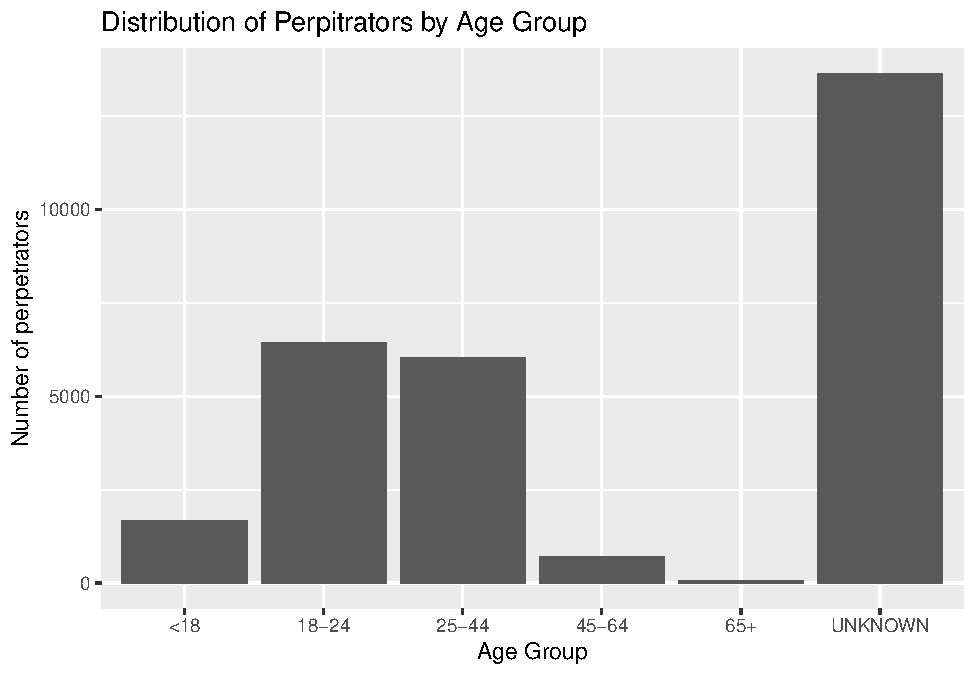
\includegraphics{nypd-shooting-data-analysis_files/figure-latex/distributions-1.pdf}

\begin{Shaded}
\begin{Highlighting}[]
\CommentTok{\# Distribution of the perpetrators by sex PERP\_SEX}
\NormalTok{shooting\_data }\SpecialCharTok{\%\textgreater{}\%}
  \FunctionTok{count}\NormalTok{(PERP\_SEX) }\SpecialCharTok{\%\textgreater{}\%}
  \FunctionTok{ggplot}\NormalTok{(}\FunctionTok{aes}\NormalTok{(}\AttributeTok{x =}\NormalTok{ PERP\_SEX, }\AttributeTok{y =}\NormalTok{ n)) }\SpecialCharTok{+}
  \FunctionTok{geom\_bar}\NormalTok{(}\AttributeTok{stat =} \StringTok{"identity"}\NormalTok{) }\SpecialCharTok{+}
  \FunctionTok{labs}\NormalTok{(}\AttributeTok{title =} \StringTok{"Distribution of Perpitrators by Sex"}\NormalTok{,}
       \AttributeTok{x =} \StringTok{"Sex"}\NormalTok{,}
       \AttributeTok{y =} \StringTok{"Number of Perpitrators"}\NormalTok{)}
\end{Highlighting}
\end{Shaded}

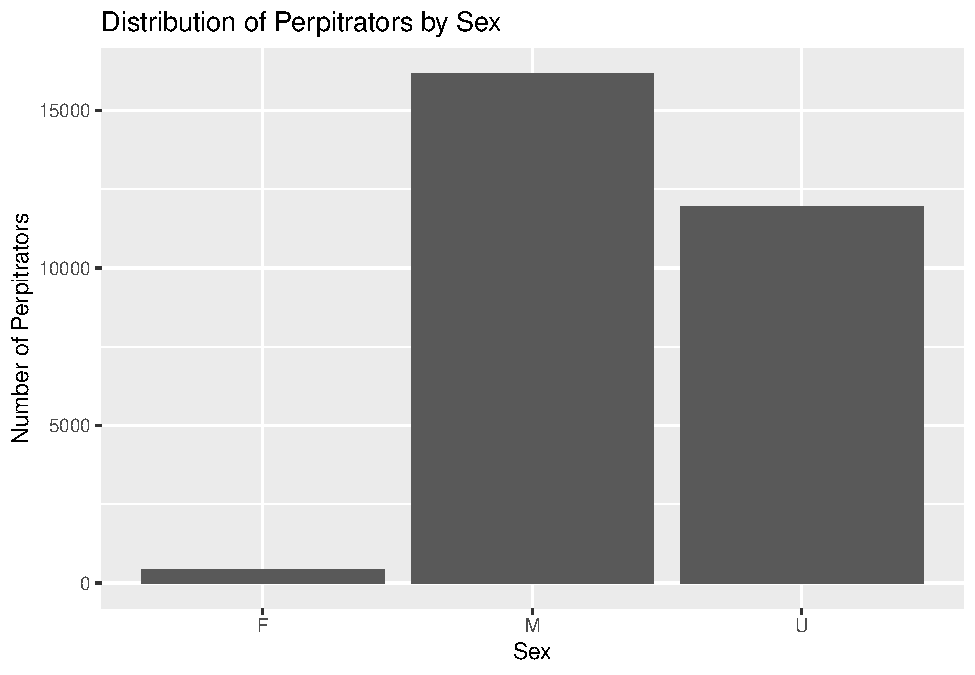
\includegraphics{nypd-shooting-data-analysis_files/figure-latex/distributions-2.pdf}

\begin{Shaded}
\begin{Highlighting}[]
\CommentTok{\# Distribution of the perpetrators by race PERP\_RACE }
\NormalTok{shooting\_data }\SpecialCharTok{\%\textgreater{}\%}
  \FunctionTok{count}\NormalTok{(PERP\_RACE) }\SpecialCharTok{\%\textgreater{}\%}
  \FunctionTok{ggplot}\NormalTok{(}\FunctionTok{aes}\NormalTok{(}\AttributeTok{x =}\NormalTok{ PERP\_RACE, }\AttributeTok{y =}\NormalTok{ n)) }\SpecialCharTok{+}
  \FunctionTok{geom\_bar}\NormalTok{(}\AttributeTok{stat =} \StringTok{"identity"}\NormalTok{) }\SpecialCharTok{+}
  \FunctionTok{labs}\NormalTok{(}\AttributeTok{title =} \StringTok{"Distribution of Perpitrators by Race"}\NormalTok{,}
       \AttributeTok{x =} \StringTok{"Race"}\NormalTok{,}
       \AttributeTok{y =} \StringTok{"Number of Perpitrators"}\NormalTok{)  }\SpecialCharTok{+}
  \FunctionTok{theme}\NormalTok{(}\AttributeTok{axis.text.x =} \FunctionTok{element\_text}\NormalTok{(}\AttributeTok{angle =} \DecValTok{45}\NormalTok{, }\AttributeTok{hjust =} \DecValTok{1}\NormalTok{))}
\end{Highlighting}
\end{Shaded}

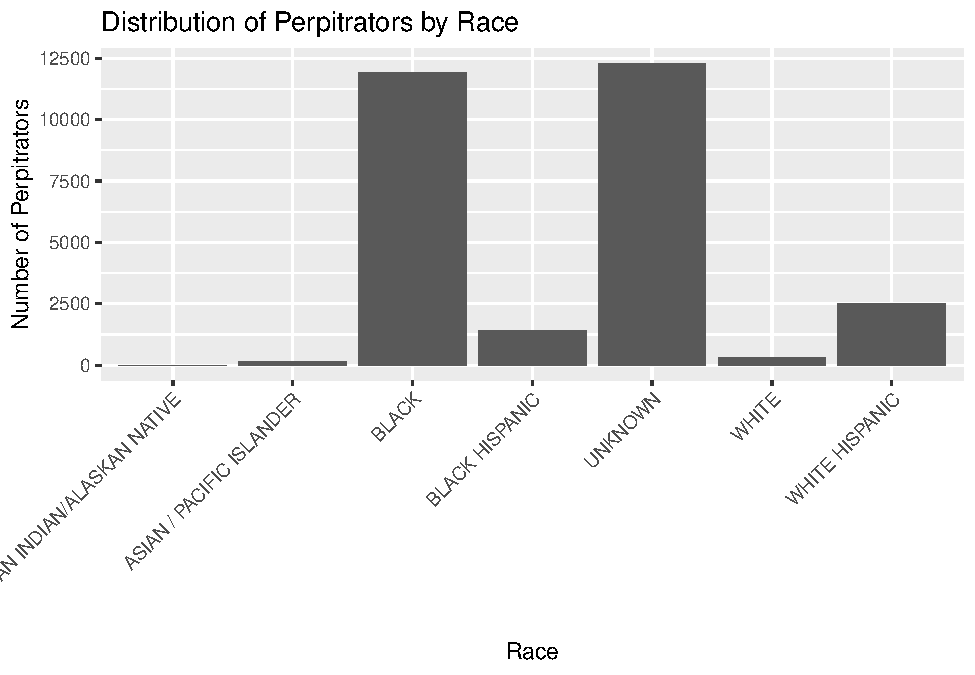
\includegraphics{nypd-shooting-data-analysis_files/figure-latex/distributions-3.pdf}

\begin{Shaded}
\begin{Highlighting}[]
\CommentTok{\# Distribution of shootings by borough BORO}
\NormalTok{shooting\_data }\SpecialCharTok{\%\textgreater{}\%}
  \FunctionTok{count}\NormalTok{(BORO) }\SpecialCharTok{\%\textgreater{}\%}
  \FunctionTok{ggplot}\NormalTok{(}\FunctionTok{aes}\NormalTok{(}\AttributeTok{x =}\NormalTok{ BORO, }\AttributeTok{y =}\NormalTok{ n)) }\SpecialCharTok{+}
  \FunctionTok{geom\_bar}\NormalTok{(}\AttributeTok{stat =} \StringTok{"identity"}\NormalTok{) }\SpecialCharTok{+}
  \FunctionTok{labs}\NormalTok{(}\AttributeTok{title =} \StringTok{"Distribution of Shootings by Borough"}\NormalTok{,}
       \AttributeTok{x =} \StringTok{"Borough"}\NormalTok{,}
       \AttributeTok{y =} \StringTok{"Number of Shootings"}\NormalTok{)  }\SpecialCharTok{+}
  \FunctionTok{theme}\NormalTok{(}\AttributeTok{axis.text.x =} \FunctionTok{element\_text}\NormalTok{(}\AttributeTok{angle =} \DecValTok{45}\NormalTok{, }\AttributeTok{hjust =} \DecValTok{1}\NormalTok{))}
\end{Highlighting}
\end{Shaded}

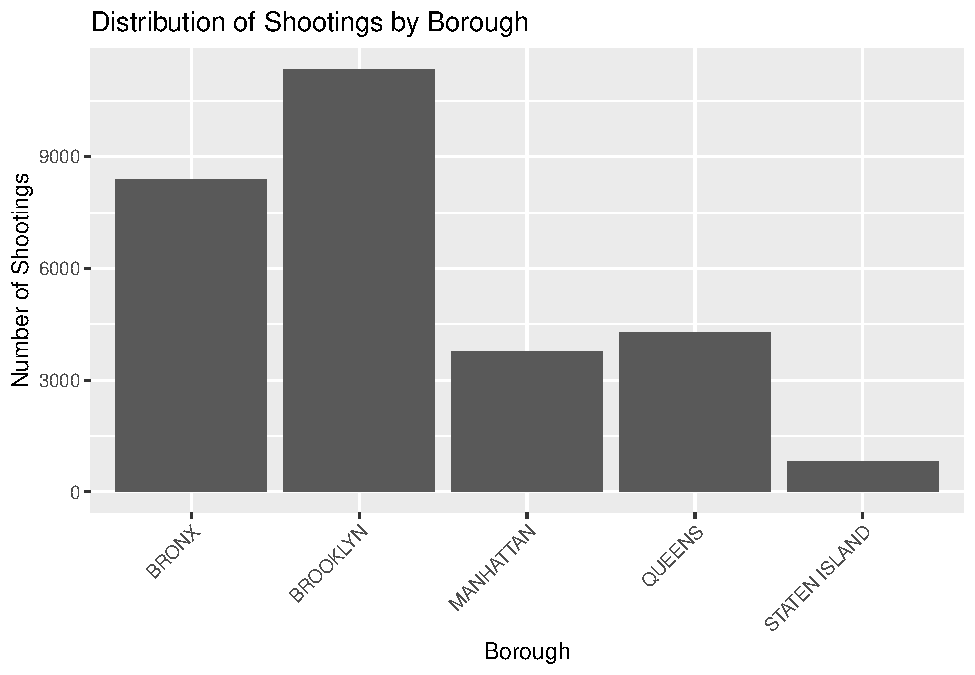
\includegraphics{nypd-shooting-data-analysis_files/figure-latex/distributions-4.pdf}

\subsubsection{Analysis}\label{analysis}

Lets take a closer look at the shootings by borough over time and see
what the trends looks like.

\begin{Shaded}
\begin{Highlighting}[]
\CommentTok{\# Create a data frame of shootings over time grouped by borough}
\NormalTok{shootings\_borough }\OtherTok{\textless{}{-}}\NormalTok{ shooting\_data }\SpecialCharTok{\%\textgreater{}\%}
  \FunctionTok{group\_by}\NormalTok{(BORO, OCCUR\_DATE) }\SpecialCharTok{\%\textgreater{}\%}
  \FunctionTok{summarise}\NormalTok{(}\AttributeTok{shootings =} \FunctionTok{n}\NormalTok{()) }\SpecialCharTok{\%\textgreater{}\%}
  \FunctionTok{select}\NormalTok{(BORO, OCCUR\_DATE, shootings) }\SpecialCharTok{\%\textgreater{}\%}
  \FunctionTok{ungroup}\NormalTok{()}
\end{Highlighting}
\end{Shaded}

\begin{verbatim}
## `summarise()` has grouped output by 'BORO'. You can override using the
## `.groups` argument.
\end{verbatim}

\begin{Shaded}
\begin{Highlighting}[]
\NormalTok{shootings\_borough}
\end{Highlighting}
\end{Shaded}

\begin{verbatim}
## # A tibble: 13,744 x 3
##    BORO  OCCUR_DATE shootings
##    <fct> <date>         <int>
##  1 BRONX 2006-01-01         2
##  2 BRONX 2006-01-04         1
##  3 BRONX 2006-01-05         2
##  4 BRONX 2006-01-06         3
##  5 BRONX 2006-01-09         4
##  6 BRONX 2006-01-10         1
##  7 BRONX 2006-01-13         2
##  8 BRONX 2006-01-14         2
##  9 BRONX 2006-01-15         2
## 10 BRONX 2006-01-16         2
## # i 13,734 more rows
\end{verbatim}

\begin{Shaded}
\begin{Highlighting}[]
\CommentTok{\# Bronx}
\NormalTok{shootings\_bronx\_monthly }\OtherTok{\textless{}{-}}\NormalTok{ shootings\_borough }\SpecialCharTok{\%\textgreater{}\%}
  \FunctionTok{filter}\NormalTok{(BORO }\SpecialCharTok{==} \StringTok{"BRONX"}\NormalTok{) }\SpecialCharTok{\%\textgreater{}\%}
  \FunctionTok{mutate}\NormalTok{(}\AttributeTok{month =} \FunctionTok{floor\_date}\NormalTok{(OCCUR\_DATE, }\AttributeTok{unit =} \StringTok{"month"}\NormalTok{)) }\SpecialCharTok{\%\textgreater{}\%}
  \FunctionTok{group\_by}\NormalTok{(month) }\SpecialCharTok{\%\textgreater{}\%}
  \FunctionTok{summarise}\NormalTok{(}\AttributeTok{shootings =} \FunctionTok{sum}\NormalTok{(shootings), }\AttributeTok{.groups =} \StringTok{"drop"}\NormalTok{)}

\FunctionTok{ggplot}\NormalTok{(shootings\_bronx\_monthly, }\FunctionTok{aes}\NormalTok{(}\AttributeTok{x =}\NormalTok{ month, }\AttributeTok{y =}\NormalTok{ shootings)) }\SpecialCharTok{+}
  \FunctionTok{geom\_line}\NormalTok{() }\SpecialCharTok{+}
  \FunctionTok{geom\_smooth}\NormalTok{(}\AttributeTok{method =} \StringTok{"loess"}\NormalTok{, }\AttributeTok{se =} \ConstantTok{FALSE}\NormalTok{, }\AttributeTok{color =} \StringTok{"red"}\NormalTok{) }\SpecialCharTok{+}
  \FunctionTok{labs}\NormalTok{(}\AttributeTok{title =} \StringTok{"Shootings in the Bronx"}\NormalTok{,}
       \AttributeTok{x =} \StringTok{"Date"}\NormalTok{,}
       \AttributeTok{y =} \StringTok{"Number of Shootings"}\NormalTok{)}
\end{Highlighting}
\end{Shaded}

\begin{verbatim}
## `geom_smooth()` using formula = 'y ~ x'
\end{verbatim}

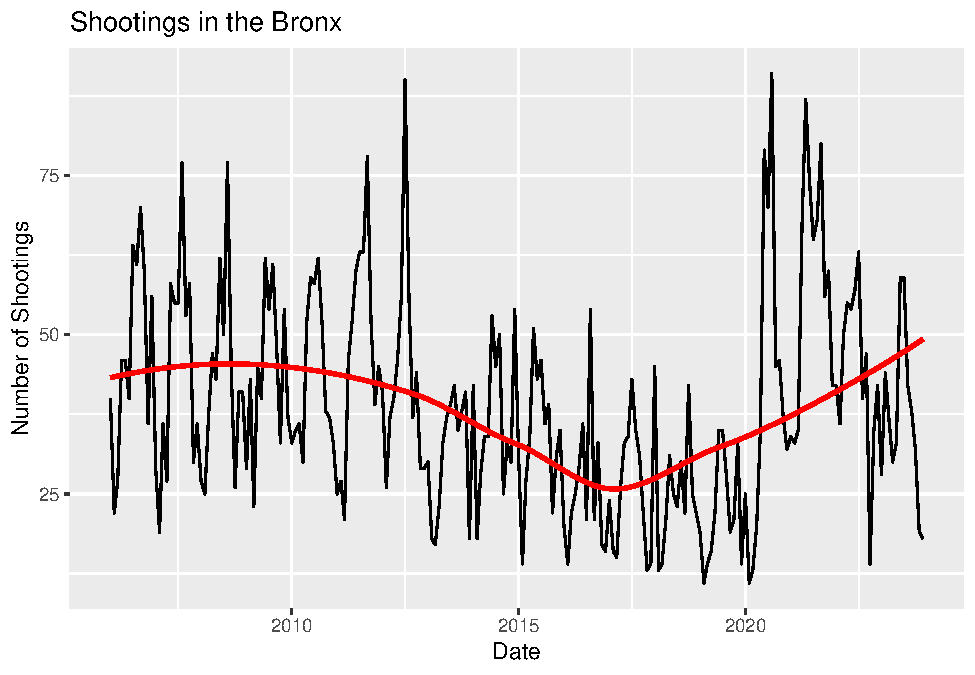
\includegraphics{nypd-shooting-data-analysis_files/figure-latex/trend-shootings-bronx-1.pdf}

\begin{Shaded}
\begin{Highlighting}[]
\CommentTok{\# Brooklyn}
\NormalTok{shootings\_brooklyn\_monthly }\OtherTok{\textless{}{-}}\NormalTok{ shootings\_borough }\SpecialCharTok{\%\textgreater{}\%}
  \FunctionTok{filter}\NormalTok{(BORO }\SpecialCharTok{==} \StringTok{"BROOKLYN"}\NormalTok{) }\SpecialCharTok{\%\textgreater{}\%}
  \FunctionTok{mutate}\NormalTok{(}\AttributeTok{month =} \FunctionTok{floor\_date}\NormalTok{(OCCUR\_DATE, }\AttributeTok{unit =} \StringTok{"month"}\NormalTok{)) }\SpecialCharTok{\%\textgreater{}\%}
  \FunctionTok{group\_by}\NormalTok{(month) }\SpecialCharTok{\%\textgreater{}\%}
  \FunctionTok{summarise}\NormalTok{(}\AttributeTok{shootings =} \FunctionTok{sum}\NormalTok{(shootings), }\AttributeTok{.groups =} \StringTok{"drop"}\NormalTok{)}

\FunctionTok{ggplot}\NormalTok{(shootings\_brooklyn\_monthly, }\FunctionTok{aes}\NormalTok{(}\AttributeTok{x =}\NormalTok{ month, }\AttributeTok{y =}\NormalTok{ shootings)) }\SpecialCharTok{+}
  \FunctionTok{geom\_line}\NormalTok{() }\SpecialCharTok{+}
  \FunctionTok{geom\_smooth}\NormalTok{(}\AttributeTok{method =} \StringTok{"loess"}\NormalTok{, }\AttributeTok{se =} \ConstantTok{FALSE}\NormalTok{, }\AttributeTok{color =} \StringTok{"red"}\NormalTok{) }\SpecialCharTok{+}
  \FunctionTok{labs}\NormalTok{(}\AttributeTok{title =} \StringTok{"Shootings in Brooklyn"}\NormalTok{,}
       \AttributeTok{x =} \StringTok{"Date"}\NormalTok{,}
       \AttributeTok{y =} \StringTok{"Number of Shootings"}\NormalTok{)}
\end{Highlighting}
\end{Shaded}

\begin{verbatim}
## `geom_smooth()` using formula = 'y ~ x'
\end{verbatim}

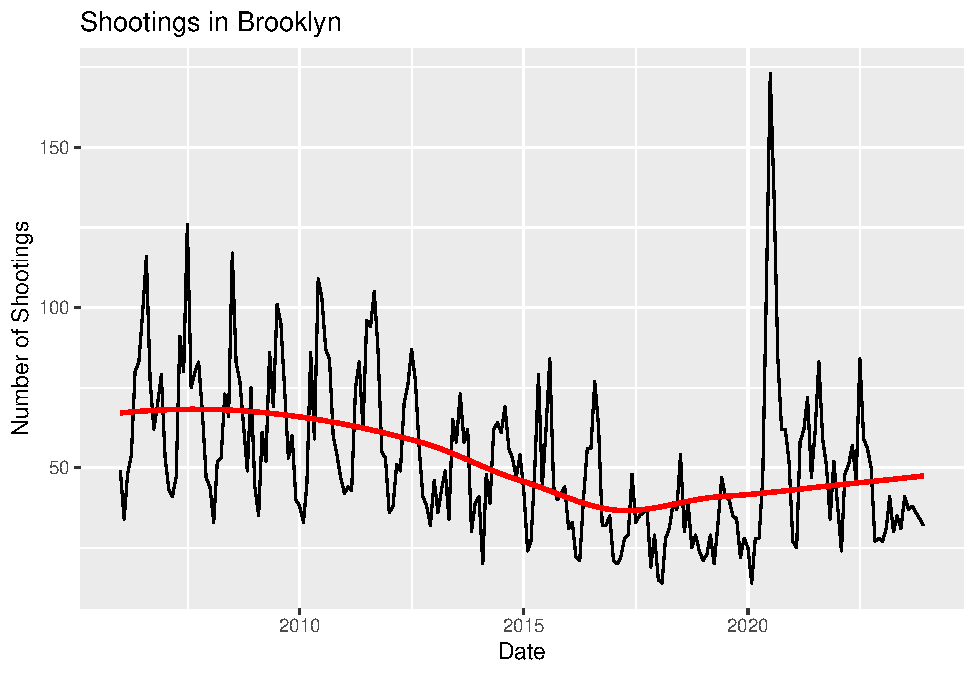
\includegraphics{nypd-shooting-data-analysis_files/figure-latex/trend-shootings-brooklyn-1.pdf}

\begin{Shaded}
\begin{Highlighting}[]
\CommentTok{\# Manhattan}
\NormalTok{shootings\_manhattan\_monthly }\OtherTok{\textless{}{-}}\NormalTok{ shootings\_borough }\SpecialCharTok{\%\textgreater{}\%}
  \FunctionTok{filter}\NormalTok{(BORO }\SpecialCharTok{==} \StringTok{"MANHATTAN"}\NormalTok{) }\SpecialCharTok{\%\textgreater{}\%}
  \FunctionTok{mutate}\NormalTok{(}\AttributeTok{month =} \FunctionTok{floor\_date}\NormalTok{(OCCUR\_DATE, }\AttributeTok{unit =} \StringTok{"month"}\NormalTok{)) }\SpecialCharTok{\%\textgreater{}\%}
  \FunctionTok{group\_by}\NormalTok{(month) }\SpecialCharTok{\%\textgreater{}\%}
  \FunctionTok{summarise}\NormalTok{(}\AttributeTok{shootings =} \FunctionTok{sum}\NormalTok{(shootings), }\AttributeTok{.groups =} \StringTok{"drop"}\NormalTok{)}

\FunctionTok{ggplot}\NormalTok{(shootings\_manhattan\_monthly, }\FunctionTok{aes}\NormalTok{(}\AttributeTok{x =}\NormalTok{ month, }\AttributeTok{y =}\NormalTok{ shootings)) }\SpecialCharTok{+}
  \FunctionTok{geom\_line}\NormalTok{() }\SpecialCharTok{+}
  \FunctionTok{geom\_smooth}\NormalTok{(}\AttributeTok{method =} \StringTok{"loess"}\NormalTok{, }\AttributeTok{se =} \ConstantTok{FALSE}\NormalTok{, }\AttributeTok{color =} \StringTok{"red"}\NormalTok{) }\SpecialCharTok{+}
  \FunctionTok{labs}\NormalTok{(}\AttributeTok{title =} \StringTok{"Shootings in the Manhattan"}\NormalTok{,}
       \AttributeTok{x =} \StringTok{"Date"}\NormalTok{,}
       \AttributeTok{y =} \StringTok{"Number of Shootings"}\NormalTok{)}
\end{Highlighting}
\end{Shaded}

\begin{verbatim}
## `geom_smooth()` using formula = 'y ~ x'
\end{verbatim}

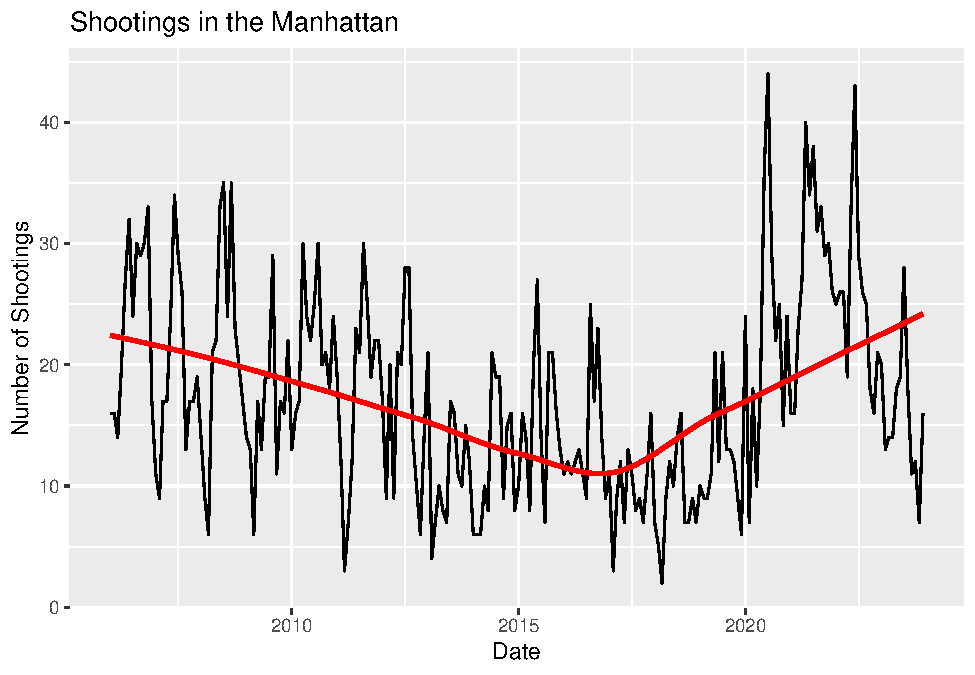
\includegraphics{nypd-shooting-data-analysis_files/figure-latex/trend-shootings-manhattan-1.pdf}

\begin{Shaded}
\begin{Highlighting}[]
\CommentTok{\# Queens}
\NormalTok{shootings\_queens\_monthly }\OtherTok{\textless{}{-}}\NormalTok{ shootings\_borough }\SpecialCharTok{\%\textgreater{}\%}
  \FunctionTok{filter}\NormalTok{(BORO }\SpecialCharTok{==} \StringTok{"QUEENS"}\NormalTok{) }\SpecialCharTok{\%\textgreater{}\%}
  \FunctionTok{mutate}\NormalTok{(}\AttributeTok{month =} \FunctionTok{floor\_date}\NormalTok{(OCCUR\_DATE, }\AttributeTok{unit =} \StringTok{"month"}\NormalTok{)) }\SpecialCharTok{\%\textgreater{}\%}
  \FunctionTok{group\_by}\NormalTok{(month) }\SpecialCharTok{\%\textgreater{}\%}
  \FunctionTok{summarise}\NormalTok{(}\AttributeTok{shootings =} \FunctionTok{sum}\NormalTok{(shootings), }\AttributeTok{.groups =} \StringTok{"drop"}\NormalTok{)}

\FunctionTok{ggplot}\NormalTok{(shootings\_queens\_monthly, }\FunctionTok{aes}\NormalTok{(}\AttributeTok{x =}\NormalTok{ month, }\AttributeTok{y =}\NormalTok{ shootings)) }\SpecialCharTok{+}
  \FunctionTok{geom\_line}\NormalTok{() }\SpecialCharTok{+}
  \FunctionTok{geom\_smooth}\NormalTok{(}\AttributeTok{method =} \StringTok{"loess"}\NormalTok{, }\AttributeTok{se =} \ConstantTok{FALSE}\NormalTok{, }\AttributeTok{color =} \StringTok{"red"}\NormalTok{) }\SpecialCharTok{+}
  \FunctionTok{labs}\NormalTok{(}\AttributeTok{title =} \StringTok{"Shootings in the Queens"}\NormalTok{,}
       \AttributeTok{x =} \StringTok{"Date"}\NormalTok{,}
       \AttributeTok{y =} \StringTok{"Number of Shootings"}\NormalTok{)}
\end{Highlighting}
\end{Shaded}

\begin{verbatim}
## `geom_smooth()` using formula = 'y ~ x'
\end{verbatim}

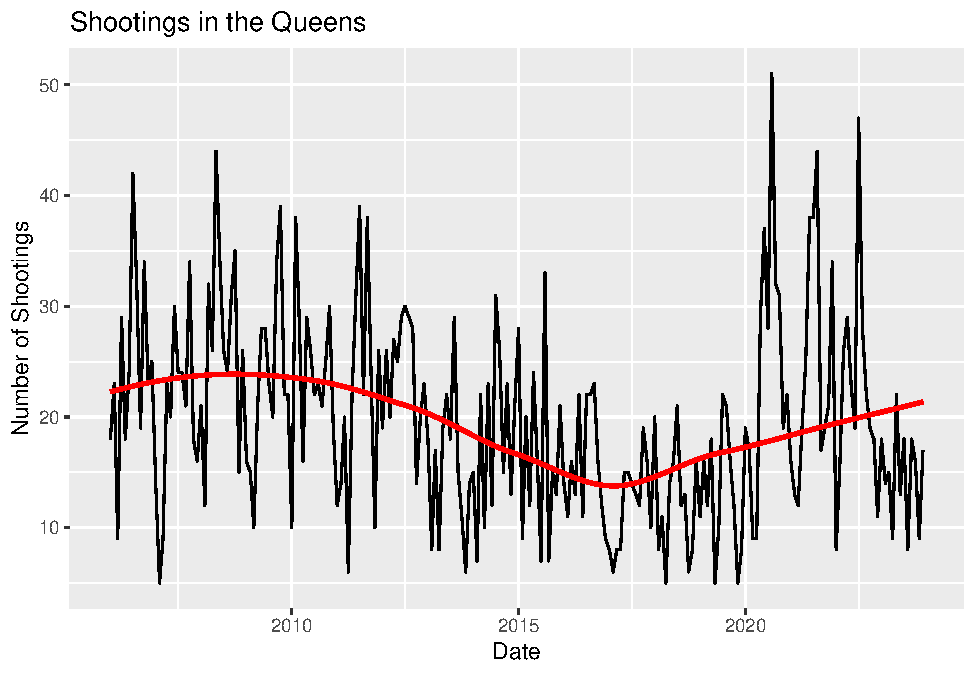
\includegraphics{nypd-shooting-data-analysis_files/figure-latex/trend-shootings-queens-1.pdf}

\begin{Shaded}
\begin{Highlighting}[]
\CommentTok{\# Staten Island}
\NormalTok{shootings\_statenisland\_monthly }\OtherTok{\textless{}{-}}\NormalTok{ shootings\_borough }\SpecialCharTok{\%\textgreater{}\%}
  \FunctionTok{filter}\NormalTok{(BORO }\SpecialCharTok{==} \StringTok{"STATEN ISLAND"}\NormalTok{) }\SpecialCharTok{\%\textgreater{}\%}
  \FunctionTok{mutate}\NormalTok{(}\AttributeTok{month =} \FunctionTok{floor\_date}\NormalTok{(OCCUR\_DATE, }\AttributeTok{unit =} \StringTok{"month"}\NormalTok{)) }\SpecialCharTok{\%\textgreater{}\%}
  \FunctionTok{group\_by}\NormalTok{(month) }\SpecialCharTok{\%\textgreater{}\%}
  \FunctionTok{summarise}\NormalTok{(}\AttributeTok{shootings =} \FunctionTok{sum}\NormalTok{(shootings), }\AttributeTok{.groups =} \StringTok{"drop"}\NormalTok{)}

\FunctionTok{ggplot}\NormalTok{(shootings\_statenisland\_monthly, }\FunctionTok{aes}\NormalTok{(}\AttributeTok{x =}\NormalTok{ month, }\AttributeTok{y =}\NormalTok{ shootings)) }\SpecialCharTok{+}
  \FunctionTok{geom\_line}\NormalTok{() }\SpecialCharTok{+}
  \FunctionTok{geom\_smooth}\NormalTok{(}\AttributeTok{method =} \StringTok{"loess"}\NormalTok{, }\AttributeTok{se =} \ConstantTok{FALSE}\NormalTok{, }\AttributeTok{color =} \StringTok{"red"}\NormalTok{) }\SpecialCharTok{+}
  \FunctionTok{labs}\NormalTok{(}\AttributeTok{title =} \StringTok{"Shootings in the Staten Island"}\NormalTok{,}
       \AttributeTok{x =} \StringTok{"Date"}\NormalTok{,}
       \AttributeTok{y =} \StringTok{"Number of Shootings"}\NormalTok{)}
\end{Highlighting}
\end{Shaded}

\begin{verbatim}
## `geom_smooth()` using formula = 'y ~ x'
\end{verbatim}

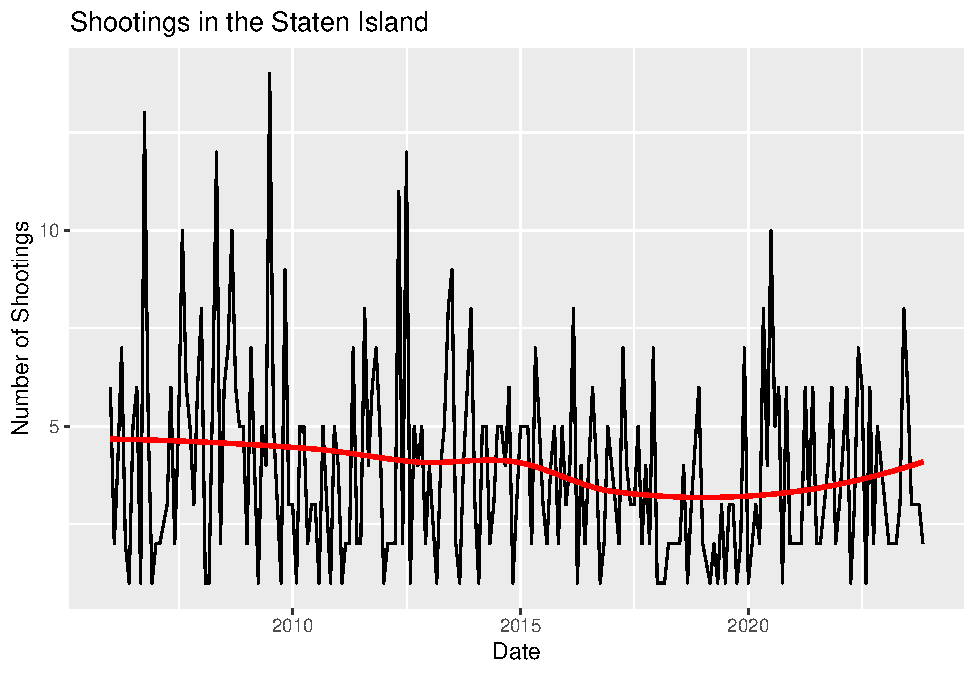
\includegraphics{nypd-shooting-data-analysis_files/figure-latex/trend-shootings-statenisland-1.pdf}
There seems to be a trend here. Let's overlay the trends for all the
boroughs to see if there's a pattern.

\begin{Shaded}
\begin{Highlighting}[]
\FunctionTok{ggplot}\NormalTok{(shootings\_borough, }\FunctionTok{aes}\NormalTok{(}\AttributeTok{x =}\NormalTok{ OCCUR\_DATE, }\AttributeTok{y =}\NormalTok{ shootings, }\AttributeTok{color =}\NormalTok{ BORO)) }\SpecialCharTok{+}
  \FunctionTok{geom\_smooth}\NormalTok{(}\AttributeTok{se =} \ConstantTok{FALSE}\NormalTok{, }\AttributeTok{method =} \StringTok{"loess"}\NormalTok{) }\SpecialCharTok{+}
  \FunctionTok{labs}\NormalTok{(}\AttributeTok{title =} \StringTok{"Monthly Shootings by Borough"}\NormalTok{,}
       \AttributeTok{x =} \StringTok{"Date"}\NormalTok{,}
       \AttributeTok{y =} \StringTok{"Number of Shootings"}\NormalTok{) }
\end{Highlighting}
\end{Shaded}

\begin{verbatim}
## `geom_smooth()` using formula = 'y ~ x'
\end{verbatim}

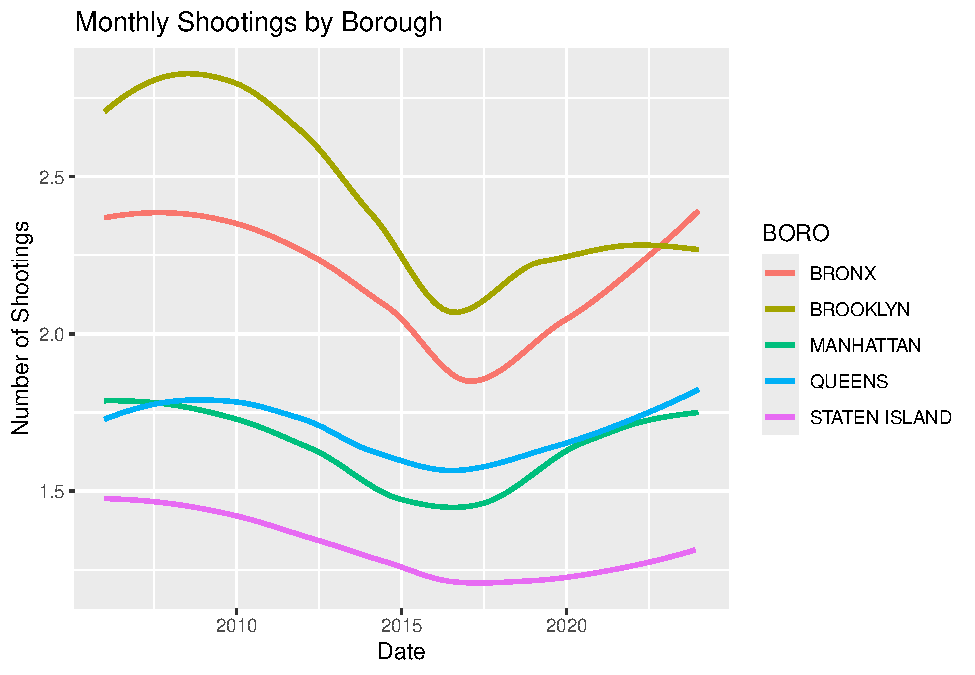
\includegraphics{nypd-shooting-data-analysis_files/figure-latex/trend-shootings-all-1.pdf}

Look at that! They all take a dip around the same time. It would be
interesting to research what was happening in the city at that time.

\subsubsection{Model}\label{model}

Lets try and predict the number of shootings in each borough by year.

\begin{Shaded}
\begin{Highlighting}[]
\NormalTok{shooting\_data}\SpecialCharTok{$}\NormalTok{Year }\OtherTok{\textless{}{-}} \FunctionTok{as.numeric}\NormalTok{(}\FunctionTok{format}\NormalTok{(shooting\_data}\SpecialCharTok{$}\NormalTok{OCCUR\_DATE, }\StringTok{"\%Y"}\NormalTok{))}

\CommentTok{\# Group by borough and year}
\NormalTok{shooting\_borough\_yearly }\OtherTok{\textless{}{-}}\NormalTok{ shooting\_data }\SpecialCharTok{\%\textgreater{}\%}
  \FunctionTok{group\_by}\NormalTok{(BORO, Year) }\SpecialCharTok{\%\textgreater{}\%}
  \FunctionTok{summarise}\NormalTok{(}\AttributeTok{Shootings =} \FunctionTok{n}\NormalTok{(), }\AttributeTok{.groups =} \StringTok{"drop"}\NormalTok{)}

\FunctionTok{head}\NormalTok{(shooting\_borough\_yearly)}
\end{Highlighting}
\end{Shaded}

\begin{verbatim}
## # A tibble: 6 x 3
##   BORO   Year Shootings
##   <fct> <dbl>     <int>
## 1 BRONX  2006       568
## 2 BRONX  2007       533
## 3 BRONX  2008       520
## 4 BRONX  2009       529
## 5 BRONX  2010       525
## 6 BRONX  2011       571
\end{verbatim}

Lets fit a simple linear model where the number of shootings is a
function of the year and borough.

\begin{Shaded}
\begin{Highlighting}[]
\CommentTok{\# Fit a simple linear model}
\NormalTok{mod }\OtherTok{\textless{}{-}} \FunctionTok{lm}\NormalTok{(Shootings }\SpecialCharTok{\textasciitilde{}}\NormalTok{ Year }\SpecialCharTok{+}\NormalTok{ BORO, }\AttributeTok{data =}\NormalTok{ shooting\_borough\_yearly)}
\FunctionTok{summary}\NormalTok{(mod)}
\end{Highlighting}
\end{Shaded}

\begin{verbatim}
## 
## Call:
## lm(formula = Shootings ~ Year + BORO, data = shooting_borough_yearly)
## 
## Residuals:
##      Min       1Q   Median       3Q      Max 
## -255.901  -47.627   -0.778   43.398  280.991 
## 
## Coefficients:
##                    Estimate Std. Error t value Pr(>|t|)    
## (Intercept)       14512.365   3943.941   3.680 0.000411 ***
## Year                 -6.973      1.958  -3.562 0.000610 ***
## BOROBROOKLYN        165.000     32.119   5.137 1.78e-06 ***
## BOROMANHATTAN      -256.333     32.119  -7.981 6.63e-12 ***
## BOROQUEENS         -228.056     32.119  -7.100 3.70e-10 ***
## BOROSTATEN ISLAND  -420.500     32.119 -13.092  < 2e-16 ***
## ---
## Signif. codes:  0 '***' 0.001 '**' 0.01 '*' 0.05 '.' 0.1 ' ' 1
## 
## Residual standard error: 96.36 on 84 degrees of freedom
## Multiple R-squared:  0.8347, Adjusted R-squared:  0.8249 
## F-statistic: 84.84 on 5 and 84 DF,  p-value: < 2.2e-16
\end{verbatim}

Lets add our predicted shootings back into our data frame.

\begin{Shaded}
\begin{Highlighting}[]
\NormalTok{shooting\_borough\_yearly}\SpecialCharTok{$}\NormalTok{Shootings\_Pred }\OtherTok{\textless{}{-}} \FunctionTok{predict}\NormalTok{(mod, shooting\_borough\_yearly)}

\FunctionTok{head}\NormalTok{(shooting\_borough\_yearly)}
\end{Highlighting}
\end{Shaded}

\begin{verbatim}
## # A tibble: 6 x 4
##   BORO   Year Shootings Shootings_Pred
##   <fct> <dbl>     <int>          <dbl>
## 1 BRONX  2006       568           525.
## 2 BRONX  2007       533           518.
## 3 BRONX  2008       520           511.
## 4 BRONX  2009       529           504.
## 5 BRONX  2010       525           497.
## 6 BRONX  2011       571           490.
\end{verbatim}

Lets visualize our predictions.

\begin{Shaded}
\begin{Highlighting}[]
\FunctionTok{ggplot}\NormalTok{(shooting\_borough\_yearly, }\FunctionTok{aes}\NormalTok{(}\AttributeTok{x =}\NormalTok{ Year, }\AttributeTok{y =}\NormalTok{ Shootings, }\AttributeTok{color =}\NormalTok{ BORO)) }\SpecialCharTok{+}
  \FunctionTok{geom\_point}\NormalTok{() }\SpecialCharTok{+}
  \FunctionTok{geom\_line}\NormalTok{(}\FunctionTok{aes}\NormalTok{(}\AttributeTok{y =}\NormalTok{ Shootings\_Pred)) }\SpecialCharTok{+}
  \FunctionTok{labs}\NormalTok{(}\AttributeTok{title =} \StringTok{"Shootings by Borough Over Time"}\NormalTok{,}
       \AttributeTok{x =} \StringTok{"Year"}\NormalTok{,}
       \AttributeTok{y =} \StringTok{"Number of Shootings"}\NormalTok{)}
\end{Highlighting}
\end{Shaded}

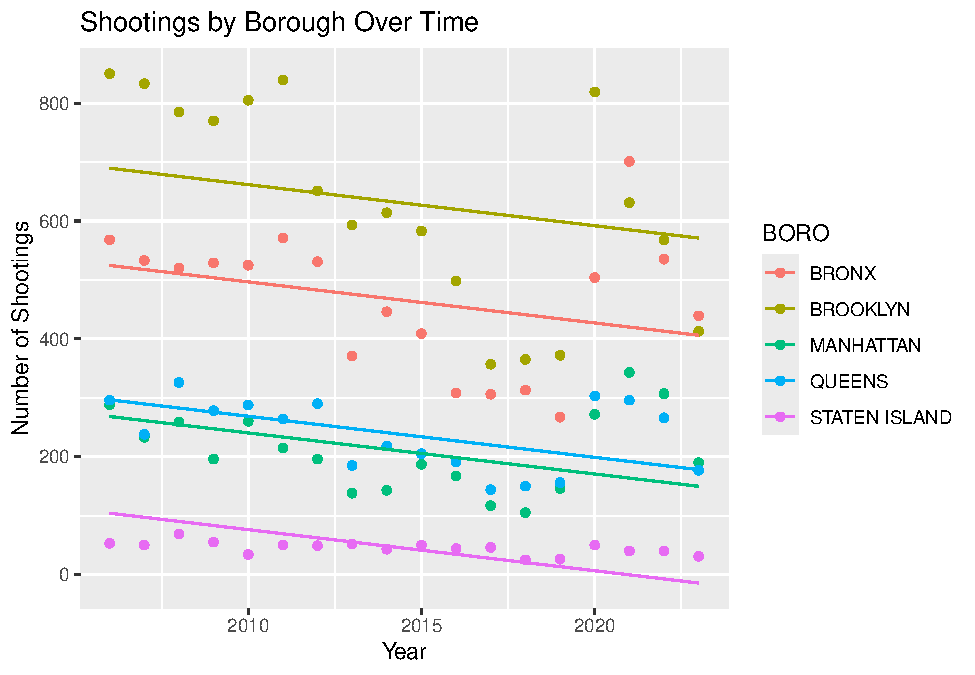
\includegraphics{nypd-shooting-data-analysis_files/figure-latex/visualize-predictions-1.pdf}

The dots show the actual number of shootings and the lines show the
predicted number of shootings. It looks like the model is a better fit
for Manhattan and Staten Island. The model also has a negative
correlation with the year. This is interesting because it suggests that
the number of shootings is decreasing over time.

\subsection{Step 4: Add Bias Identification /
Conclusion}\label{step-4-add-bias-identification-conclusion}

I think this would have been particularly relevant if I had been
investigating perpetrators. Especially since there were so many missing
values. This makes sense because they wouldn't always be able to catch
the shooter or get that information from the victim.

I live in a city (Fresno, CA) where there is a lot of crime, and
shootings are a common occurrence. I think it would be interesting to
compare the data from Fresno to the data from NY to see if there are any
similarities or differences. I am picturing NY through the lens of my
hometown and I think it would be interesting to see if the data supports
that.

\subsection{Session Info}\label{session-info}

\begin{Shaded}
\begin{Highlighting}[]
\FunctionTok{sessionInfo}\NormalTok{()}
\end{Highlighting}
\end{Shaded}

\begin{verbatim}
## R version 4.4.3 (2025-02-28 ucrt)
## Platform: x86_64-w64-mingw32/x64
## Running under: Windows 11 x64 (build 26100)
## 
## Matrix products: default
## 
## 
## locale:
## [1] LC_COLLATE=English_United States.utf8 
## [2] LC_CTYPE=English_United States.utf8   
## [3] LC_MONETARY=English_United States.utf8
## [4] LC_NUMERIC=C                          
## [5] LC_TIME=English_United States.utf8    
## 
## time zone: America/Los_Angeles
## tzcode source: internal
## 
## attached base packages:
## [1] stats     graphics  grDevices utils     datasets  methods   base     
## 
## other attached packages:
## [1] corrplot_0.95   lubridate_1.9.4 ggplot2_3.5.1   dplyr_1.1.4    
## 
## loaded via a namespace (and not attached):
##  [1] Matrix_1.7-2      gtable_0.3.6      compiler_4.4.3    tidyselect_1.2.1 
##  [5] splines_4.4.3     scales_1.3.0      yaml_2.3.10       fastmap_1.2.0    
##  [9] lattice_0.22-6    R6_2.6.1          labeling_0.4.3    generics_0.1.3   
## [13] knitr_1.49        tibble_3.2.1      munsell_0.5.1     pillar_1.10.1    
## [17] rlang_1.1.5       utf8_1.2.4        xfun_0.51         timechange_0.3.0 
## [21] cli_3.6.4         withr_3.0.2       magrittr_2.0.3    mgcv_1.9-1       
## [25] digest_0.6.37     grid_4.4.3        rstudioapi_0.17.1 lifecycle_1.0.4  
## [29] nlme_3.1-167      vctrs_0.6.5       evaluate_1.0.3    glue_1.8.0       
## [33] farver_2.1.2      colorspace_2.1-1  rmarkdown_2.29    tools_4.4.3      
## [37] pkgconfig_2.0.3   htmltools_0.5.8.1
\end{verbatim}

\end{document}
